\documentclass[12pt]{article}
\usepackage[T1]{fontenc}
\usepackage[polish]{babel}
\usepackage[utf8]{inputenc}
\usepackage{graphicx}
\usepackage{amsmath}
\usepackage{graphicx}

\graphicspath{ {./images} }


\title{Zadanie numeryczne 3}
\author{Jakub Heczko}
\date{}

\begin{document}
\section{Wstęp:}
Głownym problemem zadania jest znalezienie optymalnego algorytmu do rozwiazania naszego ukladu rownan oraz zrobienie odpowiednich optymalizacji ktore po krotce wytłumacze.Plus muszę trochę wyjaśnić syntaxę, w algorytmach, będę zakładał, że macierż jest rozmiaru N, ale na grafikach macerzy, że jest rozmiaru N+1, ale jeśli mówie, że iteruję od 0 aż do n-1 elementu to mam na myśli oczywiście dla n dużej tablicy, że iteruje od początku do końca.
\section{Optymalizacja:}
Pierwszą bardzo wazna optymalizacja jest eleminacja dzielenie przez bardzo male $h^{2}$, ponieważ wiemy, ze nasze wyrażenie $D_{2h}$ ma być równe zero to możemy bezkarnie przemnożyc przez $h^2$ co spowoduje wyeleminowanie mnożenia, nastepnie uproszczamy nasze wyrażenie i dostajemy bardzo ładna formę w postaci: 
\newline
\begin{center}
    $D_{2h} = y_{n-1} - (h^{2} - 2)y_{n} + y_{n+1}$
\end{center}
Macierz będzie wyglądać w ten sposób i bedzie miała rozmiar N+1 na N+1:
\[
\begin{bmatrix}
    1 & 0 & 0 & 0 & 0 & \dots & 0\\
    1 & h^{2}-2 & 1 & 0 & 0 & \dots & 0\\ 
    0 & 1 & h^{2}-2 & 1 & 0 & \dots & 0\\
    0 & 0 & 1 & h^{2}-2 & 1 &\dots & 0\\
    \vdots & \vdots & \vdots & \ddots & \ddots & \ddots & \vdots\\
    0 & 0 & 0 & \hdots & 1 & h^{2} & 1\\
    0 & 0 & 0 & \hdots & 0 & 0 & 1
\end{bmatrix}
*
\begin{bmatrix}
    y_{0}\\
    y_{1}\\
    y_{2}\\
    y_{3}\\
    \vdots\\
    y_{n-1}\\
    y_{n}
\end{bmatrix}
=
\begin{bmatrix}
    1\\
    0\\
    0\\
    0\\
    \vdots\\
    0\\
    0
\end{bmatrix}
\]
Jak widac bład biorący się z dzielenia został wyeleminowany, więc udało sie choć trochę zoptymalizować na poziomie juz samego zapisu i przekształceń algebraicznych. Druga optymalizacja, ktora niekoenicznie duzo daje, ale warto ja zastosowac ze wzgledu na wyglad naszej macierzy A jest odjecie od 1 woersza wiersz 0 oraz odjecie wierszu N od N-1. W ten sposob mozemy osobno obloczyc macierz takiej postaci. Będzie ona mieć rozmiar N-1 na N-1: 
\[
\begin{bmatrix}
    h^{2} & 1 & 0 & 0 & 0 & \dots & 0\\
    1 & h^{2}-2 & 1 & 0 & 0 & \dots & 0\\ 
    0 & 1 & h^{2}-2 & 1 & 0 & \dots & 0\\
    0 & 0 & 1 & h^{2}-2 & 1 &\dots & 0\\
    \vdots & \vdots & \vdots & \ddots & \ddots & \ddots & \vdots\\
    0 & 0 & 0 & \hdots & 1 & h^{2} & 1\\
    0 & 0 & 0 & \hdots & 0 & 1 & h^{2}
\end{bmatrix}
*
\begin{bmatrix}
    y_{1}\\
    y_{2}\\
    y_{3}\\
    y_{4}\\
    \vdots\\
    y_{n-2}\\
    y_{n-1}
\end{bmatrix}
=
\begin{bmatrix}
    -1\\
    0\\
    0\\
    0\\
    \vdots\\
    0\\
    0
\end{bmatrix}
\]
Mozemy tak zrobic bo mamy rozwiązane rownanie 0 oraz N, woec po odjeciu wierszy, tak jakby „podstawiliśmy” nasze rozwiazanie do poprzedniego rownania. Sprawi to ze bedziemy rozwiazaywac uklad rownan z macierza o dwa wymiary mniej poprzez uciecie dwóch wierszy i kolumn:

\section{Omówienie algorytmu Thomasa:}
Na początku przedstawie, jak analitycznie wygląda algorytm, dopiero w podsekcji, problem indeksów, pokaże, jak powinien wyglądać wzór wpisany do programy.\newline
Jak mozna poprostu zauwazyc dostajemy macierz trojdiagonalna, ktora na potrzeby zadania zapisze w 3 osobnych wektorach, jeden wektor bedzie wielkosci N i bedzie reprezentowal wartości pod diagonalą, drugi wielkosci N+1 i bedzie reprezentowal wartosci diagonalne, a trzeci podobnie jak pierwszy wielkosci N-1 i bedzie reprezentowal wartodic nad doagonala. Teraz aby optymalnie obloczyc rozwoazanoa macierzy trojdiagonalnej nalezy zastosowac algorytm thomasa, ktory daje rozwiazanie w czasie O(n).
\begin{center}
W ogólności zapiszmy nad układ jako:
$a_{i}x_{i-1} + b_{i}x_{i} + c_{i}x_{i+1} = d_{i}$ dla $i = 1,2,...,n$
\end{center}
Przy czym $a_{0} = 0$ oraz $c_{n} = 0$ czyli tak naprawde nasze skrocone wektory. Będziemy musieli póżniej uwzględnić to założenie przy naszych obliczeniach zmieniając indeksy:
Teraz załóżmy, że nasze rozwiązania można przedstawić w następujący sposób:
\begin{center}
$x_{i} = \beta_{i}x_{i+1} + \gamma_{i}$
\end{center}
A to mozna przeindeksować:
\begin{center}
$x_{i-1} = \beta_{i-1}x_{i} + \gamma_{i-1}$
\end{center}
Po odpowiednich podstawieniach pod nasze ogólne rozwiazanie $x_{i}$, dostaniemy:
\begin{center}
$\beta_{i} = \frac{c_{i}}{a_{i}\beta_{i-1}+b_{i}}$\newline\newline
$\gamma_{i} = \frac{d_{i}-a_{i}\gamma_{i-1}}{a_{i}\beta{i-1}+b_{i}}$\newline\newline
To będzie zachodzić dla $i=2,3,...,n$.
Wiemy również, że:\newline\newline
$\beta_{1} = \frac{c{1}}{b_{1}}$ ,
$\gamma_{1} = \frac{d{1}}{b_{1}}$
\end{center}
Na samym końcu naszego algorytmu trzeba jeszcze uwzlędnić krok dla n, czyli:
\begin{center}
$x_{n} = \gamma_{n}$
\end{center}
Teraz rozwiązaliśmy nasz układ w przód, musimy się jeszcze cofnąć i go rozwiązać z naszej pierwszej własności 
\begin{center}
$x_{i} = \beta_{i}x_{i+1}+\beta_{i}$ dla $i = n-1, n-2,...,1$
\end{center}
\subsection{Problem Indeksów}
Tylko tutaj pojawia się pewien problem, nasza tablica a, wielkościowo jest równa tablicy b w tym algorytmie, wiec indeksy nie beda nam sie zgadzać, trzeba więc peindeksować we wszystkich wzorach a, więc odjąć 1 w jego indeksie. Trzeba również przeindeksować sumy, bo są one dla normalnego zapisu macierzowego, czyli od każdej sumy odejmujemy 1. Dostaniemy więc końcowe wzory, które należy zaimplementować:
\begin{center}
$\beta_{i} = \frac{c_{i}}{a_{i-1}\beta_{i-1}+b_{i}}$ dla $i=1,2,...,n-2$\newline\newline Tak się dzieje ze względu na indeksy tablicy c, które należą od 0,n-2, dla n-1 kroku beta będzie poprostu równa 0, bo nie mamy już naszego c, z założen c[n-1] = 0
\end{center}
\begin{center}
$\gamma_{i} = \frac{d_{i}-a_{i-1}\gamma_{i-1}}{a_{i-1}\beta{i-1}+b_{i}}$ dla $i=1,2,...,n-1$.\newline\newline
\end{center}
Teraz rozwiązaliśmy nasz układ w przód, musimy się jeszcze cofnąć i go rozwiązać z naszej pierwszej własności 
\begin{center}
$x_{i} = \beta_{i}x_{i+1}+\gamma_{i}$ dla $i = n-2, n-1,...,0$
\end{center}
Tego typu zmiany indeksowe trzeba uwzględnić wszędzie, bo nie będziemy indeksować od 1,2,...,n, ale od 0,1,2,...,n-1.
Dokladna pesymistyczna zlozonosc to O(3N)
\section{Omówienie wyników:}
 
Jak dalej mozna zauwazyć zmierzylem czas i względne porownanałem dla bardzo duzych danych te dwie wartości, przykładowe wyniki przedstawiam na dole:
\begin{center}
Solved matrixA with numpy no efficent with time: 0.01951313018798828
\newline
\newline
Solved matrixA with thomas algorithm in time: 0.0011038780212402344
\newline
\newline
Porownanie wzgledne czasu LU do czasu thomasa:
17.676889848812095
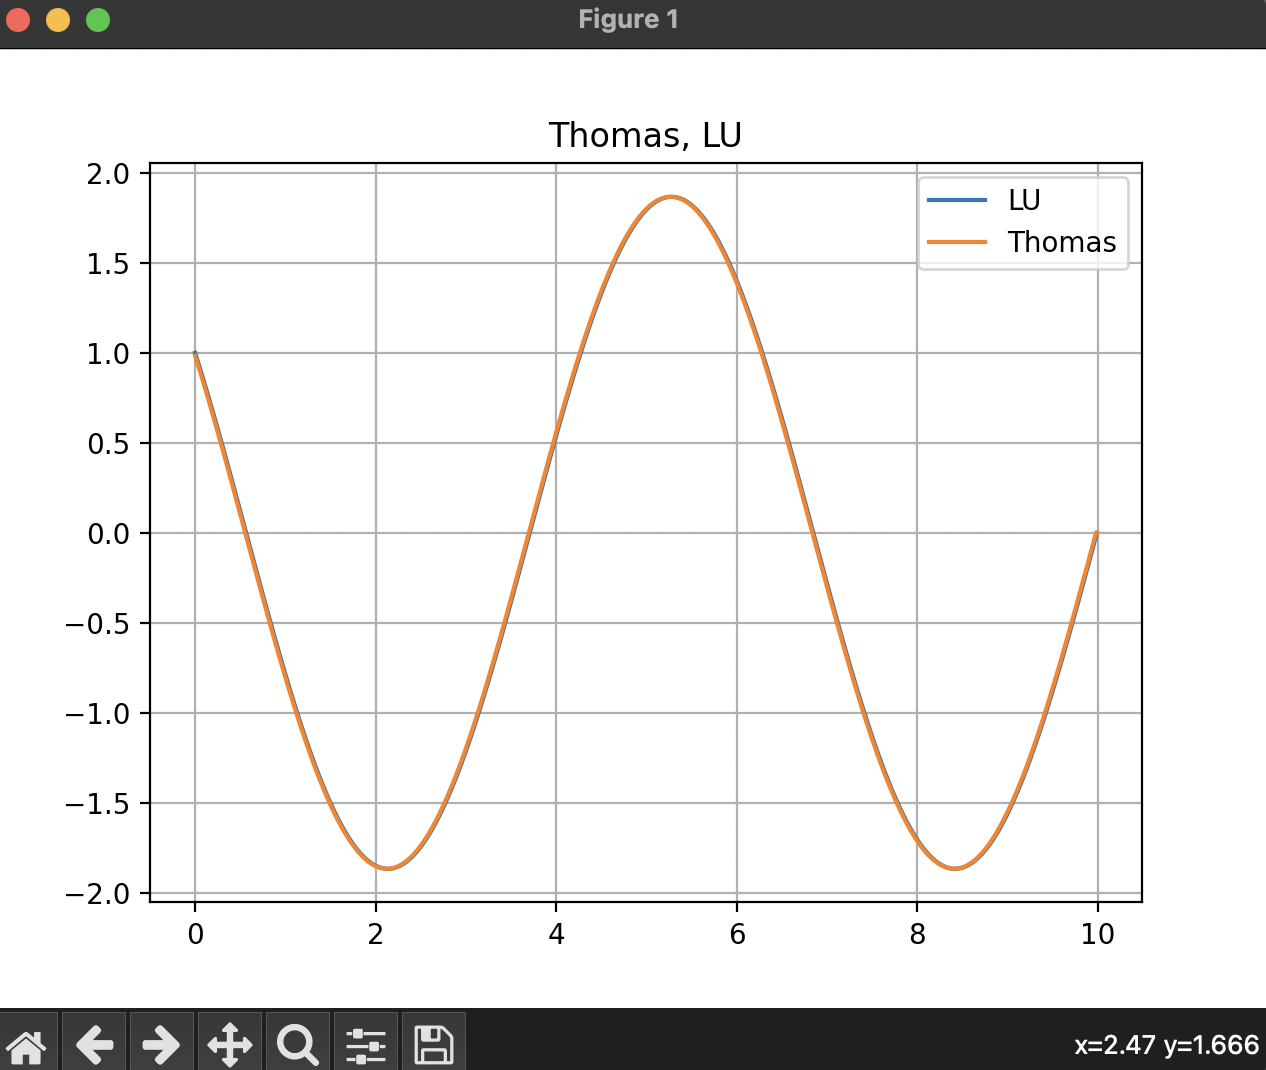
\includegraphics[width=13cm,height=8cm, keepaspectratio]{wykres}
\end{center}

\end{document}